\documentclass[11pt,a4paper]{article}
\usepackage[T1]{fontenc}
\usepackage[utf8]{inputenc}
\usepackage{geometry}
\geometry{margin=2.2cm}
\usepackage{amsmath,amssymb,bm}
\usepackage{booktabs}
\usepackage{array}
\usepackage{xcolor}
\usepackage{tikz}
\usetikzlibrary{arrows.meta,positioning,fit,backgrounds,calc,shapes.geometric}
\usepackage[ruled,vlined,linesnumbered]{algorithm2e}
\usepackage{caption}
\usepackage{enumitem}

\definecolor{seal}{RGB}{20,90,160}
\definecolor{good}{RGB}{28,128,64}
\definecolor{bad}{RGB}{178,40,40}
\definecolor{boxb}{RGB}{233,241,250}
\definecolor{boxg}{RGB}{232,245,236}
\definecolor{boxy}{RGB}{252,246,228}
\definecolor{gray2}{RGB}{120,120,120}

\usepackage{hyperref}
\hypersetup{colorlinks=true,linkcolor=seal,urlcolor=seal,citecolor=seal}

\newcommand{\good}[1]{\textcolor{good}{#1}}
\newcommand{\bad}[1]{\textcolor{bad}{#1}}

\title{\textbf{SEAL: Diagnosis-Driven SAR Ship Instance Segmentation}\\[5pt]
\large The \textbf{GeoField} Unified Geometry-Field Operator --- Evidence, Rationale, and Method}
\author{SEAL Project --- Technical Note}
\date{\today}

\begin{document}
\maketitle

\begin{abstract}
\noindent
The inshore accuracy of SAR ship instance segmentation has long been limited, and the dominant
response is to \textbf{keep adding capacity} (stronger backbones, orientation-aware queries,
foundation-model priors, diffusion decoders) --- yet a more basic question is rarely answered: for a
given strong baseline, \emph{where} does inshore fail --- are ships not found, or are found ships
poorly masked? This work follows a \textbf{diagnose-before-fix} discipline. We first use a
\emph{capacity-independent}, AP-additive oracle to decompose the inshore AP$_{75}$ deficit into a
\textbf{mask-quality} half and a \textbf{detection-coverage} half, and a size-resolved analysis
localizes the \emph{medium-object shape/boundary} deficit as the largest recoverable pool that
resolution-style remedies cannot reach. A leakage audit then shows that the evaluation split can
\emph{distort the diagnosis itself}. Guided by this diagnosis, we \textbf{borrow} the principles of
several proven mechanisms (salience reweighting, shape-adaptive sampling, absolute position,
inter-instance relation) and \textbf{redesign}, from first principles, a single native operator,
\textbf{GeoField}: each pixel computes \emph{one} shared geometry code from which an oriented sampling
kernel, a salience that is \emph{structurally inseparable} from the sampling, and a position phase are
\emph{simultaneously} derived --- mathematically entangled, not stacked. It \textbf{enriches} the shared
mask feature rather than competing with the readout in logit space, so it cannot regress the way a rigid
prior did. Throughout, an \textbf{equal-parameter control} separates ``mechanism gain'' from ``raw
capacity.'' This note gives the full evidence chain and rationale, with a framework diagram, algorithm
pseudocode, and the equal-parameter ladder.
\end{abstract}

\section{Problem and Motivation}
SAR ship instance segmentation is evaluated chiefly on PSeg-SSDD and HRSID with an inshore/offshore
stratification (the field's de-facto standard). Inshore, ships abut quays, cranes, and other man-made
metallic clutter, and accuracy collapses. The two strongest current methods --- the diffusion-based
DiffSARShipInst and the orientation-enhanced O$^2$Former --- are \textbf{both built on ResNet-50 with a
Mask2Former-style decoder}; each \emph{adds capacity} and reports aggregate or stratified AP, but
\textbf{none} performs an attribution of \emph{where} the inshore deficit arises. Our carrier (denoted
A0) is exactly Mask2Former-R50, the recognized field baseline.

\section{Core Idea: Diagnose Before Fix}
We hold one methodological principle: \textbf{the diagnosis is the protagonist; a mechanism is a
falsifiable corollary of the diagnosis.} Without first quantifying \emph{which axis} the deficit lies
on, no architectural gain can be attributed to the mechanism it claims, and effort may target a
sub-problem that is not the binding constraint. The full logical chain is shown in
Fig.~\ref{fig:arc}; each step takes the unique exit forced by the previous one as its entry.

\begin{figure}[h]
\centering
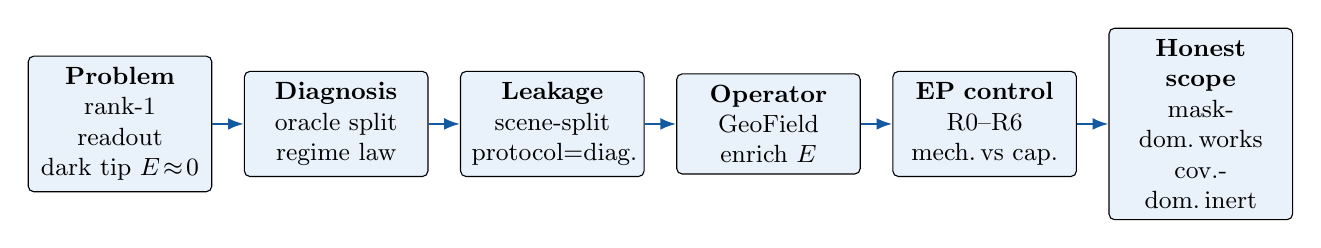
\begin{tikzpicture}[
  node distance=4mm,
  stage/.style={draw,rounded corners=2pt,fill=boxb,inner sep=4pt,align=center,font=\small,text width=2.05cm,minimum height=1.1cm},
  arr/.style={-{Latex[length=2mm]},seal,thick}]
\node[stage] (p) {\textbf{Problem}\\rank-1 readout\\dark tip $E\!\approx\!0$};
\node[stage,right=of p] (d) {\textbf{Diagnosis}\\oracle split\\regime law};
\node[stage,right=of d] (l) {\textbf{Leakage}\\scene-split\\protocol$=$diag.};
\node[stage,right=of l] (o) {\textbf{Operator}\\GeoField\\enrich $E$};
\node[stage,right=of o] (v) {\textbf{EP control}\\R0--R6\\mech.\,vs cap.};
\node[stage,right=of v] (s) {\textbf{Honest scope}\\mask-dom.\,works\\cov.-dom.\,inert};
\draw[arr] (p)--(d); \draw[arr] (d)--(l); \draw[arr] (l)--(o);
\draw[arr] (o)--(v); \draw[arr] (v)--(s);
\end{tikzpicture}
\caption{SEAL's argumentative spine: diagnosis-driven, equal-parameter-controlled, scope-honest.}
\label{fig:arc}
\end{figure}

\section{Diagnostic Evidence}
\paragraph{(1) AP-additive oracle decomposition (capacity-independent).} On the A0 carrier, holding
detection fixed and substituting \emph{literal ground-truth masks}, we re-run COCO evaluation to obtain
the recoverable \emph{ceiling} of inshore AP$_{75}$. Result: the inshore deficit is \textbf{about half
mask-quality and half detection-coverage} --- not ``mask is the sole bottleneck,'' but a
\textbf{regime-dependent two-way constraint}.

\paragraph{(2) Regime law (five points).} Tabulating base AP$_{75}$, mask share, and coverage share by
dataset/stratum (Table~\ref{tab:regime}): lower base $\Rightarrow$ more coverage-dominated; mask share
falls with difficulty.

\begin{table}[h]\centering\small
\caption{The regime-dependent two-way constraint (mask\% / coverage\%).}
\label{tab:regime}
\begin{tabular}{lccc}
\toprule
Stratum & base AP$_{75}$ & mask\% & coverage\% \\
\midrule
PSeg inshore        & 0.341 & 51 & 49 \\
PSeg all            & 0.615 & 69 & 31 \\
PSeg offshore       & 0.735 & 87 & 13 \\
HRSID official (leak) & 0.378 & 43 & 57 \\
HRSID scene (leak-free) & 0.206 & \textbf{23} & \textbf{77} \\
\bottomrule
\end{tabular}
\end{table}

\paragraph{(3) Size-resolved decomposition --- locating the target.} Stratifying the mask-quality
oracle by object size gives the recoverable AP$_{75}$:
\begin{equation}
\text{small } \;+0.253,\qquad \boxed{\text{medium }\;+0.394}\;(\text{largest}),\qquad \text{large } \;+0.000\,(\text{saturated}).
\end{equation}
The \textbf{medium-object recoverable pool is the largest}; yet the resolution-style refinement head
below \emph{only reaches small} (a small object spans $\sim$5 mask pixels at $1/4$ stride --- it is
resolution-limited) and is \textbf{inert on medium}. The medium deficit is therefore one of
\emph{shape/boundary detail} and needs a different lever --- precisely GeoField's target axis.

\paragraph{(4) Leakage audit --- protocol welded to diagnosis.} The official HRSID split has heavy chip
leakage; the leak-free \emph{scene-level} split is the truth. Leakage not only inflates AP but
\textbf{disguises ``coverage-dominated'' (23\% mask) as ``balanced'' (43\% mask)} --- \emph{without
fixing leakage, one even mis-judges which axis binds}. All cross-dataset claims must therefore run on
the leak-free scene-split.

\section{Negative Results and Lessons (keep the essence, discard the dross)}
The value of the diagnostic discipline is that it \textbf{rejected several of our own well-motivated
designs} on the spot --- these NO-GOs are the basis for the subsequent design and the collateral for
the paper's credibility.

\begin{itemize}[leftmargin=1.2em,itemsep=2pt]
\item \bad{ShapePrior / GeoKernel (NO-GO)}: a gated rigid oriented-ellipse prior added in
\emph{logit space}, $M_q=\sigma(e_q\!\cdot\!E+g\,P)$. Across three seeds it \textbf{regressed the
baseline} (geo $0.597 <$ blind $0.609 <$ baseline $0.638$), and geo did not beat blind. Root cause:
\textbf{a rigid prior fights the optimized rank-1 readout}. $\Rightarrow$ \good{Lesson: enrich, do not
compete.}
\item \bad{DAOM-Seed (inert)}: a training-time one-to-many auxiliary seeding was indistinguishable from
its content-matched null, and both regressed. $\Rightarrow$ \good{Lesson: a relational/auxiliary
mechanism must beat its own null to count.}
\item \good{Refinement head (PASS, honestly attributed)}: PSeg overall AP$_{75}$ \textbf{$+3.0$
(3-seed mean)}; an \emph{equal-parameter control} proves the gain is \textbf{capacity, not resolution}
(caps$=$refine$=0.643 \gg$ bilinear $0.628$). It recovers small and is inert on medium. $\Rightarrow$
\good{Lesson: an equal-parameter control can refute the authors' own narrative.}
\end{itemize}

\section{Borrow and Redesign}
We \textbf{do not stack modules}. We distill several proven mechanisms into \emph{principles} and
redesign them, from first principles, into \emph{one} operator (Table~\ref{tab:principle}). Its lineage
traces to a self-validated semantic-segmentation teacher (UNet++, with a CoordConv mask head, dynamic
snake convolution, CBAM, BatchFormer), but \textbf{one cannot point to those modules in the graph} ---
there is only a bottleneck, a shared code, and a set of free bases.

\begin{table}[h]\centering\small
\caption{Four principles $\to$ read-outs of one shared computation (why it is a redesign, not a stack).}
\label{tab:principle}
\renewcommand{\arraystretch}{1.15}
\begin{tabular}{>{\raggedright\arraybackslash}p{2.7cm}>{\raggedright\arraybackslash}p{6.3cm}>{\raggedright\arraybackslash}p{4.6cm}}
\toprule
Principle (lineage) & Form inside GeoField & Inseparability \\
\midrule
CBAM $\to$ salience & $s_p=\sigma(a\,e_p+\rho_p)$, $e_p=\lVert E_{\text{mix}}-E\rVert$ & \textbf{no own projection --- to ablate $s$ you must remove kernel $k$} \\
DSConv $\to$ shape sampling & per-pixel oriented kernel $k_p$ from a free low-rank basis $\{B^m\}$ & predicted weights, not offset-gather; not Gaussian/harmonic \\
CoordConv $\to$ position & coords enter the bottleneck before the code, plus phase $\rho_p$ & into the feature, not the logit \\
BatchFormer $\to$ relation & \emph{training-only} RKD relational regularizer on the code & zero inference params, batch-independent \\
\bottomrule
\end{tabular}
\end{table}

\section{GeoField: a Unified Geometry-Field Operator}
\subsection{Landing site and non-regression}
A Mask2Former mask is the rank-1 readout $M_q=\sigma(e_q\!\cdot\!E)$: each query vector $e_q$ is dotted
with a \emph{shared} per-pixel feature $E$, with \textbf{no per-instance spatial degree of freedom}, so
the low-backscatter dark bow/stern ($E\!\approx\!0$) is systematically under-segmented. GeoField
\textbf{enriches} that shared feature:
\begin{equation}
E' = E + \gamma\cdot s_p \odot E_{\text{mix}},
\end{equation}
feeding the \emph{unchanged} same readout $\langle e_q, E'\rangle$ (detection and segmentation share
$E'$, ensuring coherence). It \textbf{never adds to logit space}, and the residual gate $\gamma$ is
LayerScale-initialized to $0$, so at step 0 it is \emph{byte-identical in output} to the baseline
refinement head --- structurally it cannot repeat the rigid prior's regression / numerical collapse.

\subsection{Framework and internal structure}
Fig.~\ref{fig:pipe} shows the overall framework and where GeoField sits (Plan A head-slot; Plan B
threaded into the pixel decoder). Fig.~\ref{fig:op} shows the operator internally --- ``one shared code
$\to$ three entangled read-outs.''

\begin{figure}[h]
\centering
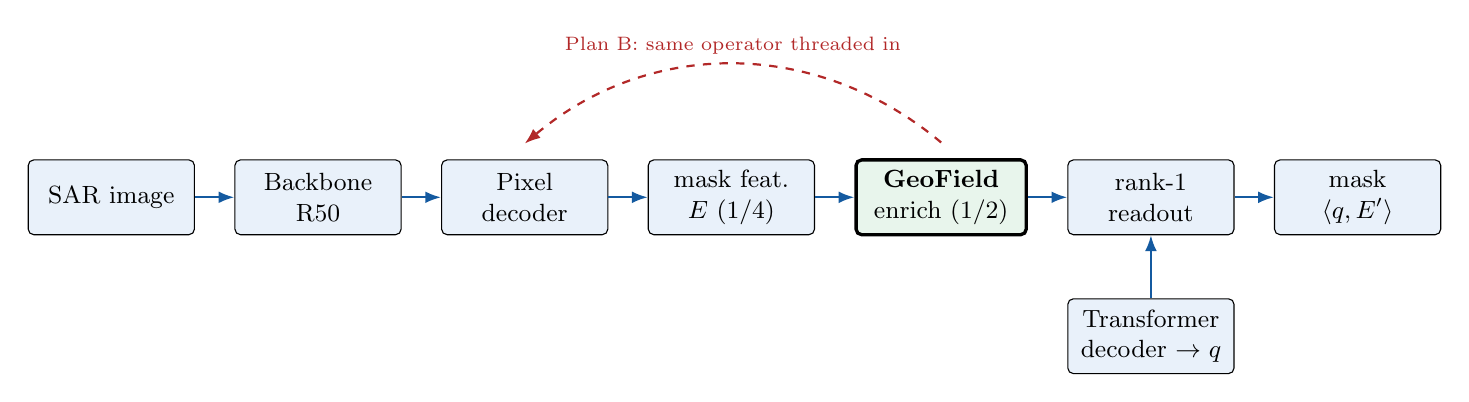
\begin{tikzpicture}[
  node distance=5mm,
  blk/.style={draw,rounded corners=2pt,fill=boxb,inner sep=3pt,align=center,font=\small,minimum height=0.95cm,text width=1.9cm},
  gf/.style={draw,rounded corners=2pt,fill=boxg,very thick,inner sep=3pt,align=center,font=\small,minimum height=0.95cm,text width=1.95cm},
  arr/.style={-{Latex[length=2mm]},seal,thick}]
\node[blk] (img) {SAR image};
\node[blk,right=of img] (bb) {Backbone\\R50};
\node[blk,right=of bb] (pd) {Pixel decoder};
\node[blk,right=of pd] (E) {mask feat.\\$E$ (1/4)};
\node[gf,right=of E] (gf) {\textbf{GeoField}\\enrich (1/2)};
\node[blk,right=of gf] (rd) {rank-1\\readout};
\node[blk,below=8mm of rd] (q) {Transformer\\decoder $\to q$};
\node[blk,right=of rd] (m) {mask\\$\langle q,E'\rangle$};
\draw[arr] (img)--(bb); \draw[arr] (bb)--(pd); \draw[arr] (pd)--(E);
\draw[arr] (E)--(gf); \draw[arr] (gf)--(rd); \draw[arr] (rd)--(m);
\draw[arr] (q)--(rd);
\draw[arr,dashed,bad] ($(gf.north)+(0,2mm)$) to[out=140,in=40] node[above,font=\scriptsize,bad]{Plan B: same operator threaded in} ($(pd.north)+(0,2mm)$);
\end{tikzpicture}
\caption{Overall framework. GeoField enriches the shared feature $E$ in the head-slot (Plan A, solid);
Plan B threads the \emph{same} operator into the pixel-decoder input (dashed), at the same depth as the
field's network-level co-adaptation.}
\label{fig:pipe}
\end{figure}

\begin{figure}[h]
\centering
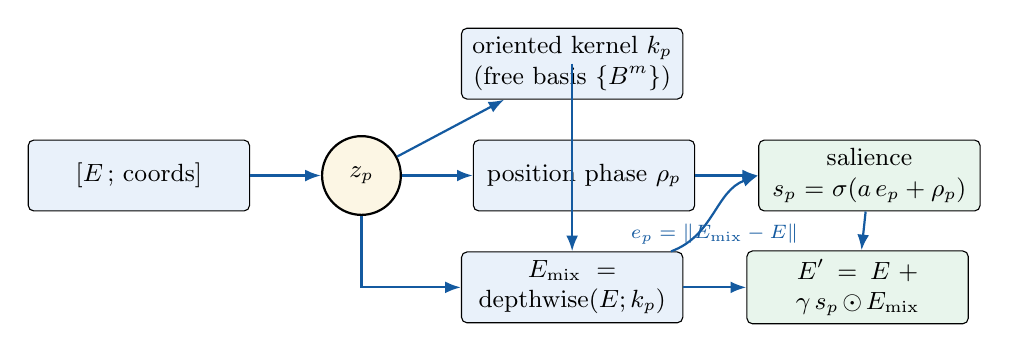
\begin{tikzpicture}[
  node distance=6mm and 9mm,
  zsty/.style={draw,circle,fill=boxy,thick,inner sep=1pt,font=\small,minimum size=1.0cm},
  rd/.style={draw,rounded corners=2pt,fill=boxb,inner sep=3pt,align=center,font=\small,text width=2.6cm,minimum height=0.9cm},
  op/.style={draw,rounded corners=2pt,fill=boxg,inner sep=3pt,align=center,font=\small,text width=2.6cm,minimum height=0.9cm},
  arr/.style={-{Latex[length=2mm]},seal,thick}]
\node[rd] (in) {$[E\,;\,\text{coords}]$};
\node[zsty,right=of in] (zc) {$z_p$};
\node[rd,above right=of zc] (k) {oriented kernel $k_p$\\(free basis $\{B^m\}$)};
\node[rd,right=of zc] (rho) {position phase $\rho_p$};
\node[rd,below right=of zc] (mix) {$E_{\text{mix}}=$\\depthwise$(E;k_p)$};
\node[op,right=8mm of rho] (s) {salience\\$s_p=\sigma(a\,e_p+\rho_p)$};
\node[op,right=8mm of mix] (out) {$E'=E+\gamma\,s_p\!\odot\!E_{\text{mix}}$};
\draw[arr] (in)--(zc);
\draw[arr] (zc)--(k); \draw[arr] (zc)--(rho); \draw[arr] (zc)|-(mix);
\draw[arr] (k)-|(mix.north);
\draw[arr] (mix) to[out=20,in=200] node[below,font=\scriptsize]{$e_p=\lVert E_{\text{mix}}-E\rVert$} (s.west);
\draw[arr] (rho)--(s);
\draw[arr] (s)--(out); \draw[arr] (mix)--(out);
\end{tikzpicture}
\caption{Inside GeoField: a single shared code $z_p$ simultaneously yields the oriented sampling kernel,
the position phase, and the salience; salience is set by the kernel-mix residual energy $e_p$ and is
thus \textbf{structurally inseparable} from the sampling.}
\label{fig:op}
\end{figure}

\subsection{Algorithm (pseudocode)}
\begin{algorithm}[h]
\small
\SetKwInOut{Input}{Input}\SetKwInOut{Output}{Output}
\caption{GeoField forward (gen\_mode selects the ladder arm)}
\label{alg:gf}
\Input{feature $E\in\mathbb{R}^{B\times C\times H\times W}$; mode $\in\{$off,\,capacity,\,pos,\,shape,\,full$\}$}
\Output{enriched feature $E'$ (same shape)}
\If{mode $=$ off}{\Return $E$\;}
$\text{coords}\leftarrow$ normalized $(x,y)\in[-1,1]$; zero them if $\neg$use\_pos\;
$z \leftarrow W_1\,\mathrm{SiLU}(\mathrm{GN}(W_0[E;\text{coords}]))$ \tcp*{the one shared geometry code (1$\times$1 bottleneck)}
\eIf{use\_shape}{
  $\alpha\leftarrow W_k z$; $\;k \leftarrow \mathrm{softmax}_{ij}\!\big(\textstyle\sum_m \alpha_m B^m\big)$ \tcp*{free-basis oriented kernel, fp32}
}{
  $k \leftarrow$ isotropic uniform kernel $\tfrac{1}{K^2}$ \tcp*{shape off}
}
$E_{\text{mix}}\leftarrow \sum_{i,j} k_{ij}\cdot \mathrm{shift}_{ij}(E)$ \tcp*{$K\times K$ shift-accumulate, memory $O(BCHW)$}
$\rho \leftarrow \tanh(W_{\text{pos}} z)$\;
\eIf{use\_shape}{$e_p\leftarrow \lVert E_{\text{mix}}-E\rVert_2$; $\;s\leftarrow \sigma(a\,e_p+\rho)$ \tcp*{salience $\equiv$ kernel energy}}{$s\leftarrow \sigma(\rho)$\;}
\Return $E + \gamma\, s \odot E_{\text{mix}}$ \tcp*{$\gamma$ init $0$ $\Rightarrow$ identity}
\end{algorithm}

\section{Equal-Parameter Ladder}
One class, one \texttt{gen\_mode} switch, \textbf{byte-identical parameters} ($21{,}698{,}148$ per arm,
measured); the switch only changes the forward computation (zero the coordinates, freeze the kernel to
isotropic, degrade salience to a content gate) and \emph{adds/removes no parameters}.

\begin{table}[h]\centering\small
\caption{Equal-parameter ladder and decision criteria (target = the medium stratum).}
\label{tab:ladder}
\begin{tabular}{llp{6.6cm}}
\toprule
Arm & Name & What it isolates / criterion \\
\midrule
R0 & off & bypass $=$ stock refinement head (sanity) \\
R1 & capacity & pure capacity (constant coords, isotropic kernel, free content gate)\\
R2 & pos & $+$ position (answers ``is the sine PE already enough?'')\\
R3 & shape & $+$ oriented free-basis kernel $+$ shape-coupled salience \\
R5 & full & the complete operator (note: \textbf{no R4 salience-only by construction} = novelty evidence)\\
R6 & full+rel & $+$ training-only RKD relation (inference params identical to R5)\\
\midrule
\multicolumn{3}{l}{\textbf{Criteria}: \good{fusion$>$capacity $\Leftrightarrow$ R5$>$R1}; \;\good{entanglement $\Leftrightarrow$ R5$>\max($R2,R3$)$}; \;\good{relation $\Leftrightarrow$ R6$>$R5} (all over multi-seed bootstrap CIs)}\\
\bottomrule
\end{tabular}
\end{table}

\noindent\textbf{Why medium is the target:} (i) the oracle says the medium recoverable mask pool is the
largest ($+0.394$); (ii) the refinement head is inert on medium --- a \emph{shape}, not resolution,
problem, exactly what GeoField attacks; (iii) \textbf{capacity is inert on medium} (in the pilot,
R1$\approx$R0), so any R5 gain on medium is \emph{attributable to the mechanism alone} --- the
equal-parameter control has its sharpest discriminating power on this axis.

\section{Co-Adaptation (more than the head)}
Field SOTA all \textbf{modify the baseline network}, not just the mask head: O$^2$Former co-adapts at
the \emph{feature input} (direction-aware convolution before the pixel decoder) and \emph{query
initialization}; DiffSARShipInst modifies the neck/loss/mask-reconstruction. Therefore:
\begin{itemize}[leftmargin=1.2em,itemsep=2pt]
\item \textbf{Plan A (current)}: GeoField enriches the refined $E$ in the head-slot, for a
\emph{cheap, controlled} mechanism test.
\item \textbf{Plan B (after GO)}: thread the \emph{same} operator into the \textbf{pixel-decoder input}
--- the diagnosis says the $E\!\approx\!0$ dark tip \emph{originates upstream}, so this is the
highest-value co-adaptation site, at the same depth as O$^2$Former, but \emph{unifying} its
``fixed-angle rotation branches $+$ polar encoding'' with a single shared-code free-basis kernel.
\end{itemize}

\section{Current Evidence (verification status)}
\begin{table}[h]\centering\small
\caption{Completed verifications (measured).}
\label{tab:evidence}
\begin{tabular}{lp{8.6cm}c}
\toprule
Item & Result & Status \\
\midrule
Operator CPU smoke & equal-param / residual-identity / finite fwd+bwd / AMP-stable / \textbf{batch-independent} ($2.4\!\times\!10^{-7}$) / arm-differentiation & \good{7/7 pass} \\
Head-level equal-param & all six arms $21{,}698{,}148$ params (byte-identical) & \good{pass} \\
GPU training smoke & R5, real data, 12 iters: loss monotonically down, no NaN/OOM, 8.6\,GB & \good{pass} \\
Deployment verification & ONNX export / torch-ONNX-TensorRT parity ($4.8\!\times\!10^{-7}$) / batch-independent & \good{pass} \\
Deployment FPS & reference impl is memory-bound (fp32 $\approx 1.5\times$ a plain conv); fused kernel is future work & \textcolor{gray2}{honestly logged} \\
4-arm pilot (PSeg) & R0/R1 done (medium mAP $0.444/0.441$, capacity inert on medium); R3/R5 in progress & \textcolor{gray2}{in progress} \\
\bottomrule
\end{tabular}
\end{table}

\section{Story and Positioning}
SEAL \textbf{shares the same baseline} (Mask2Former-R50) with the two 2025 SOTA methods, but pursues a
\emph{diagnosis-driven, equal-parameter-controlled, scope-honest} co-adaptation rather than SOTA-chasing.
The key narrative is that \textbf{the diagnosis is the protagonist}: whether the GeoField pilot is a
strong win, a capacity result, or a tie, the paper stands --- a strong win is ``diagnosis $\to$ targeted
design $\to$ mechanism gain attributed by the equal-parameter control''; a tie is ``even a
diagnosis-targeted operator cannot beat the control $\Rightarrow$ it strengthens the two-way-constraint
thesis.'' The predicted inertness on the coverage-dominated HRSID is the diagnosis \emph{correctly
predicting} that mask-side help should not transfer, reported as a \emph{declared negative-transfer
control}. We do \textbf{not} claim to beat competitors on raw AP at $14\times$ fewer epochs; the
contribution is the \emph{diagnostic methodology $+$ the unified operator $+$ the leakage audit}.

\vspace{4pt}
\noindent\rule{\linewidth}{0.4pt}\\[2pt]
{\footnotesize Note: all numbers are verified measured/oracle values; the pilot arms R3/R5 are still
training, and the verdict will be updated once available.}

\end{document}
